%!TEX root = project.tex

\chapter*{About this project}
\paragraph{Abstract}

TBC...

\paragraph{Authors}
Damian Nolan, Daniel Verdejo



\chapter{Introduction}
Any person providing an online personal consultancy services always face the challenge of acquiring, managing and retaining clients and delivery of the service over a disparate array of tools.  The primary problem is fragmentation of these tools.  Social media platforms such as Facebook are great in providing the networking and promotional aspect of things and while it is possible to run a business this way it is not the most effective and efficient means to an end.  Furthermore they are not designed to be business focused.
The goal is to streamline the experience and allow a service provider to focus on the service delivery and growing their consultancy rather than having a inordinate amount of time managing clients. Consider the following user stories:
\begin{itemize}
\item When deciding to offer an online service that involves interpersonal communication, Users want to be able to setup a personal page describing my services, so that I can manage the communication from the point of purchase right through to delivering my online service.
\item When users setup personal pages describing their services, Users want to be able to set their pricing and the times they are normally willing to provide services, so that a user can feel like they are in control of their consultancy and their client knows when they are ordinarily available.
\item When a user decides to avail of an online service that involves interpersonal communication, they want to be able to pay and have their account created if they do not already have one, additionally have their first session scheduled for them, so that they can manage their schedule accordingly.
\item A consultant will be able to setup an online consultancy within ten minutes without training and receive their renumeration for work completed within thirty days without having to chase up with clients for outstanding invoicing.  Additionally a client won’t have to waste any time chasing up with the consultant on asking how to pay for the service.  Double booking of clients should not be a problem as the system should provide adequate feedback when this is likely to occur. 
\end{itemize}

\chapter{Context}
\begin{itemize}
\item Provide a context for your project.
\item Set out the objectives of the project
\item Briefly list each chapter / section and provide a 1-2 line description of what each section contains.
\item List the resource URL (GitHub address) for the project and provide a brief list of the main elements at the URL.
\end{itemize}

\section{Filler}


\subsection{More filler}


\section{Filler}


\chapter{Methodology}
\section{Kanban Management Approach}
Throughout the development life-cycle for this project we implemented an Agile Kanban task management approach. Kanban is a management method that enables teams and organizations to visualize their work, outline and reduce or completely remove bottlenecks, and achieve significant operational advancements in terms of quality and throughput\cite{kanban}. The methodology aims to gradually improve any aspect of an organization, whether it be IT/operations, software development and engineering, staffing, marketing and so on. The core concept of Kanban are the following:
\begin{itemize}
\item Visualize Workflow
	\begin{itemize}
	\item Separate the complete workload into descriptive segments or states, visualized as named columns on a wall.
    \item Write each user story (piece of work) on to a card and place in a column to indicate how far along the workflow the piece of work is
  	\end{itemize}
\item Limit Work In Progress
	\begin{itemize}
	\item Allocate specific limits to how many pieces of work can be in progress within each workflow segment or state.
	\end{itemize}
\item Measure the Lead Time
	\begin{itemize}
	\item Lead Time, also referred to as cycle time, is the average time required to complete one piece of work. Measure Lead Time and optimize the process to make the Lead Time as predictable and small as possible.
	\end{itemize}
\end{itemize}

This may look somewhat familiar if you are knowledgeable in the Lean Pull Scheduling System, as Kanban is a direct implementation of this\cite{kanban}. A piece of work can only progress to the next segment or state when it acquires a slot in there.The implementation of Kanban and other Lean Manufacturing Methods, can significantly benefit workflow in some of the following ways:

\begin{itemize}
\item Visibility of bottlenecks become very apparent in real-time. This promotes collaboration amongst people to optimize the entire value chain as opposed to just their own part.
\item Tends to Naturally grow throughout all aspects of the organization, resulting in higher visibility of all goings on within the organization.
\item Reduces company costs via reduction of inventory within the range of 25\%-75\%.
\item Continuous support, and increased speed of all pieces of work within the workflow due to visibilty and organization.
\end{itemize}

Kanban supports continuous workflow, termed Value Stream, when it is applied as a project management approach to software development projects. "The Value Stream consists of all actions required to bring a project from creation to completion."\cite{kanban}. Actions can either add value to the project, or add no value, but may or may not be avoidable. When an action is avoidable it is termed as waste, the elimination of waste is facilitated by the Kanban methodology. In software development terms, there are three types of waste:
\begin{itemize}
\item Waste in code development, due to
	\begin{itemize}
	\item Partially completed work, Defects.
	\end{itemize}
\item Waste in project management, due to
	\begin{itemize}
	\item Extra processes, code hand offs, extra functions.
	\end{itemize}
\item Waste in team potential, due to
	\begin{itemize}
	\item Task switching, waiting for information or instructions.
	\end{itemize}
\end{itemize}

\section{Agile Kanban with Git Workflow}
Agile Kanban is a Kanban approach to Agile Software Development. In Agile Kanban, the Kanban board is used as a visualization of the workflow. The board will display the status and progress being made on individual tasks, where they can be tracked. Consider Figure \ref{fig:kanban}

\paragraph{}
Git workflow as a version control tool is a system that tracks modifications to a file or files over the lifetime of a project so that a developer or team can recall specific versions at a later stage. A very common version-control method is to copy files from one directory to another directory. This method is common because it is easy, but is incredibly error prone. It is easy to mistake the directory that is currently active and accidentally write to the incorrect file or copy over files that were not intended to be.\cite{chachon} The main difference between Git and other version control software tools is the way Git handles its data. Where other systems use what is often referred to as delta-based version control, they store information as a set of files and the changes made to each file over time, Git does not  store its data this way. Instead, Git stores its data more like a collection of snapshots of a miniature file system. In Git, whenever a commit is made, a picture of what all the files look like at that point in time is taken and stored as a reference to that snapshot.\cite{chachon} If any of the files have not been changed, Git does not store the file again, just a pointer to the previous file it has already collected and stored. "Git thinks about its data more like a stream of snapshots."\cite{chachon}



\begin{figure}
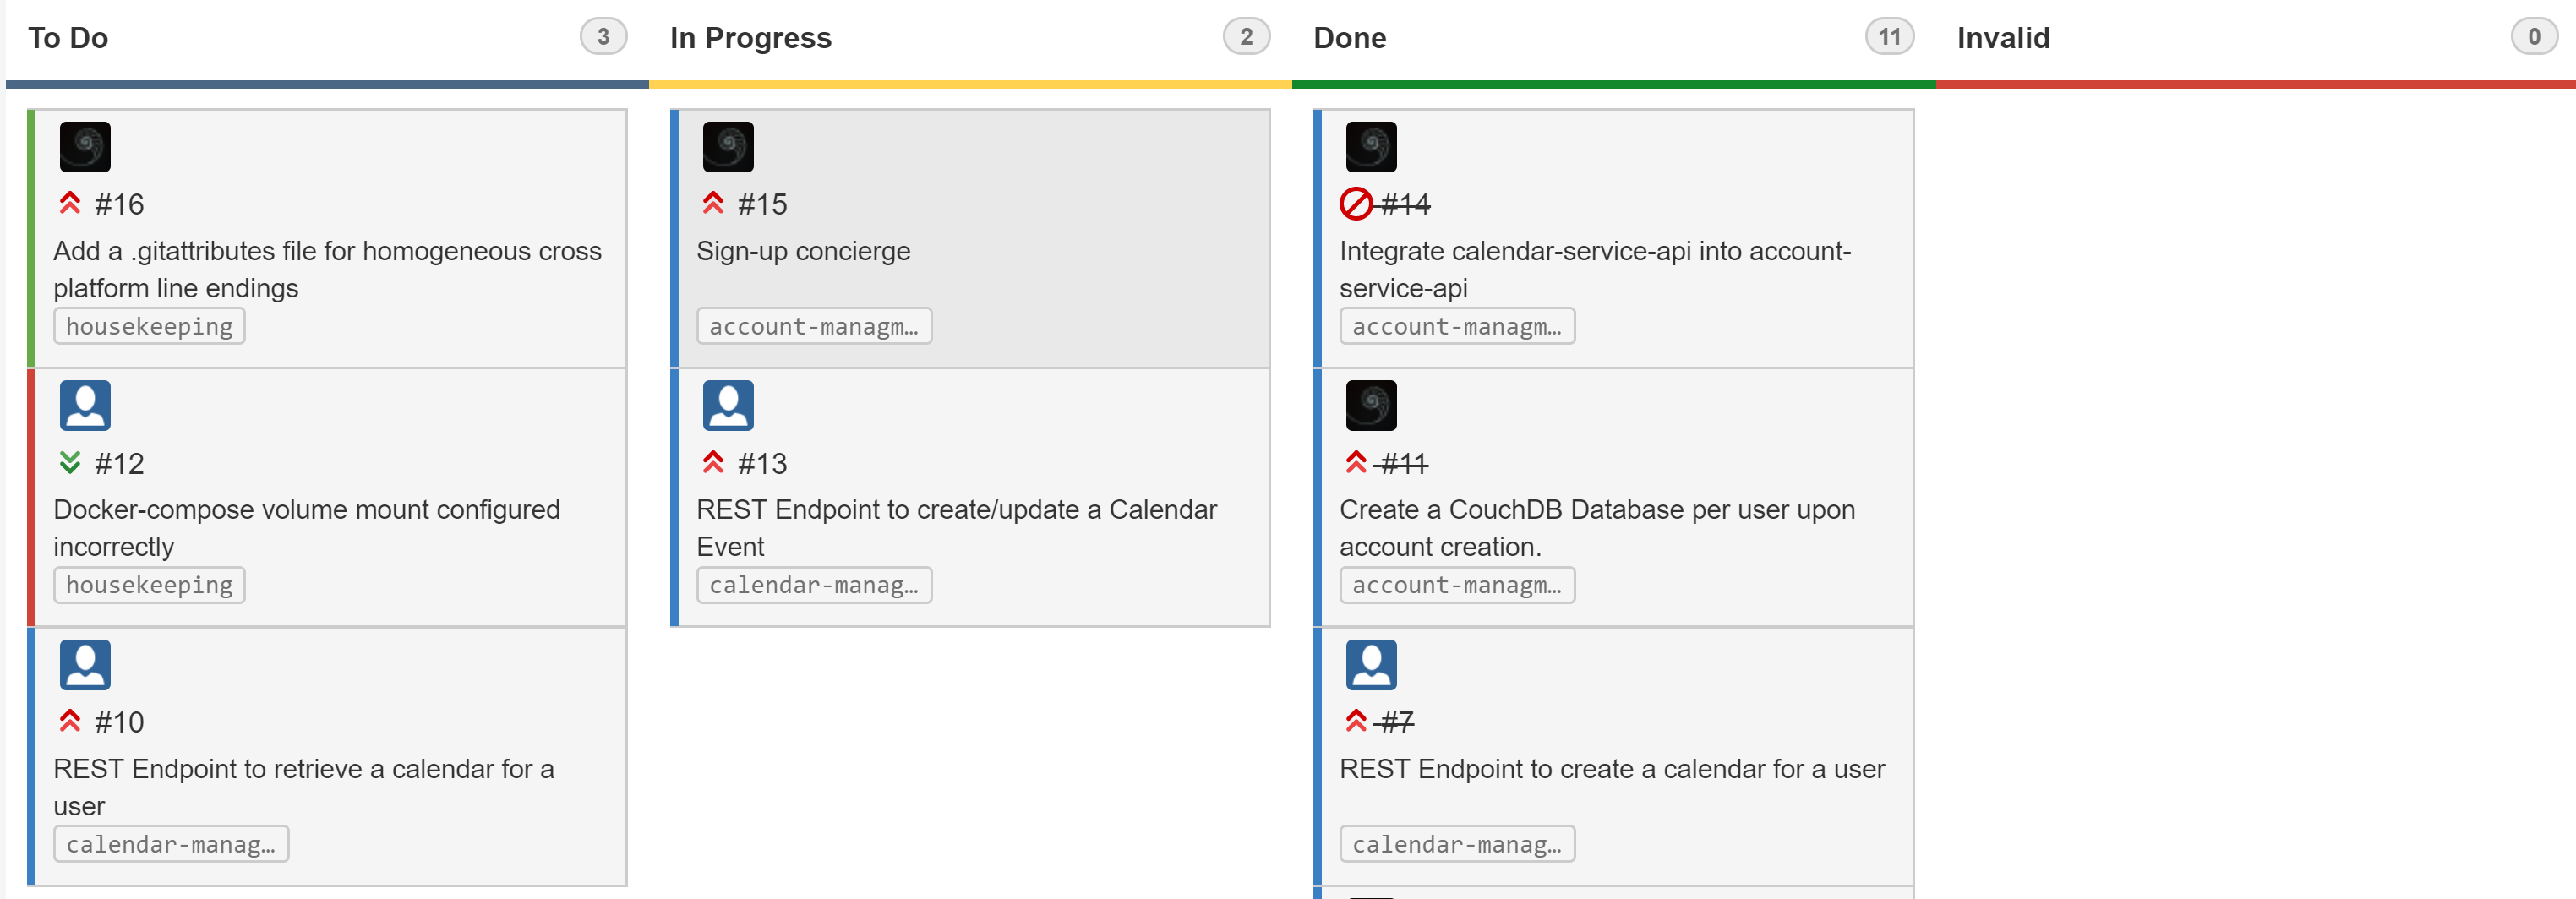
\includegraphics[width=\textwidth]{img/Kanban.PNG}
\caption{Kanban Board}
\label{fig:kanban}
\end{figure}

\paragraph{}In the Figure \ref{fig:kanban} example a couple of tasks have been created, each given their priority as well as the component they relate to and displayed on the board in the To Do state. A developer can come and move a task from the To Do state into the In Progress state to signify that this task is now being worked on. In order to protect the main development / master branch from becoming corrupted by merge conflicts, where numerous developers may be editing the same segment of work, when a task is started a new branch is created off of the development branch\cite{driessen}. See \ref{fig:branches}

\begin{figure}
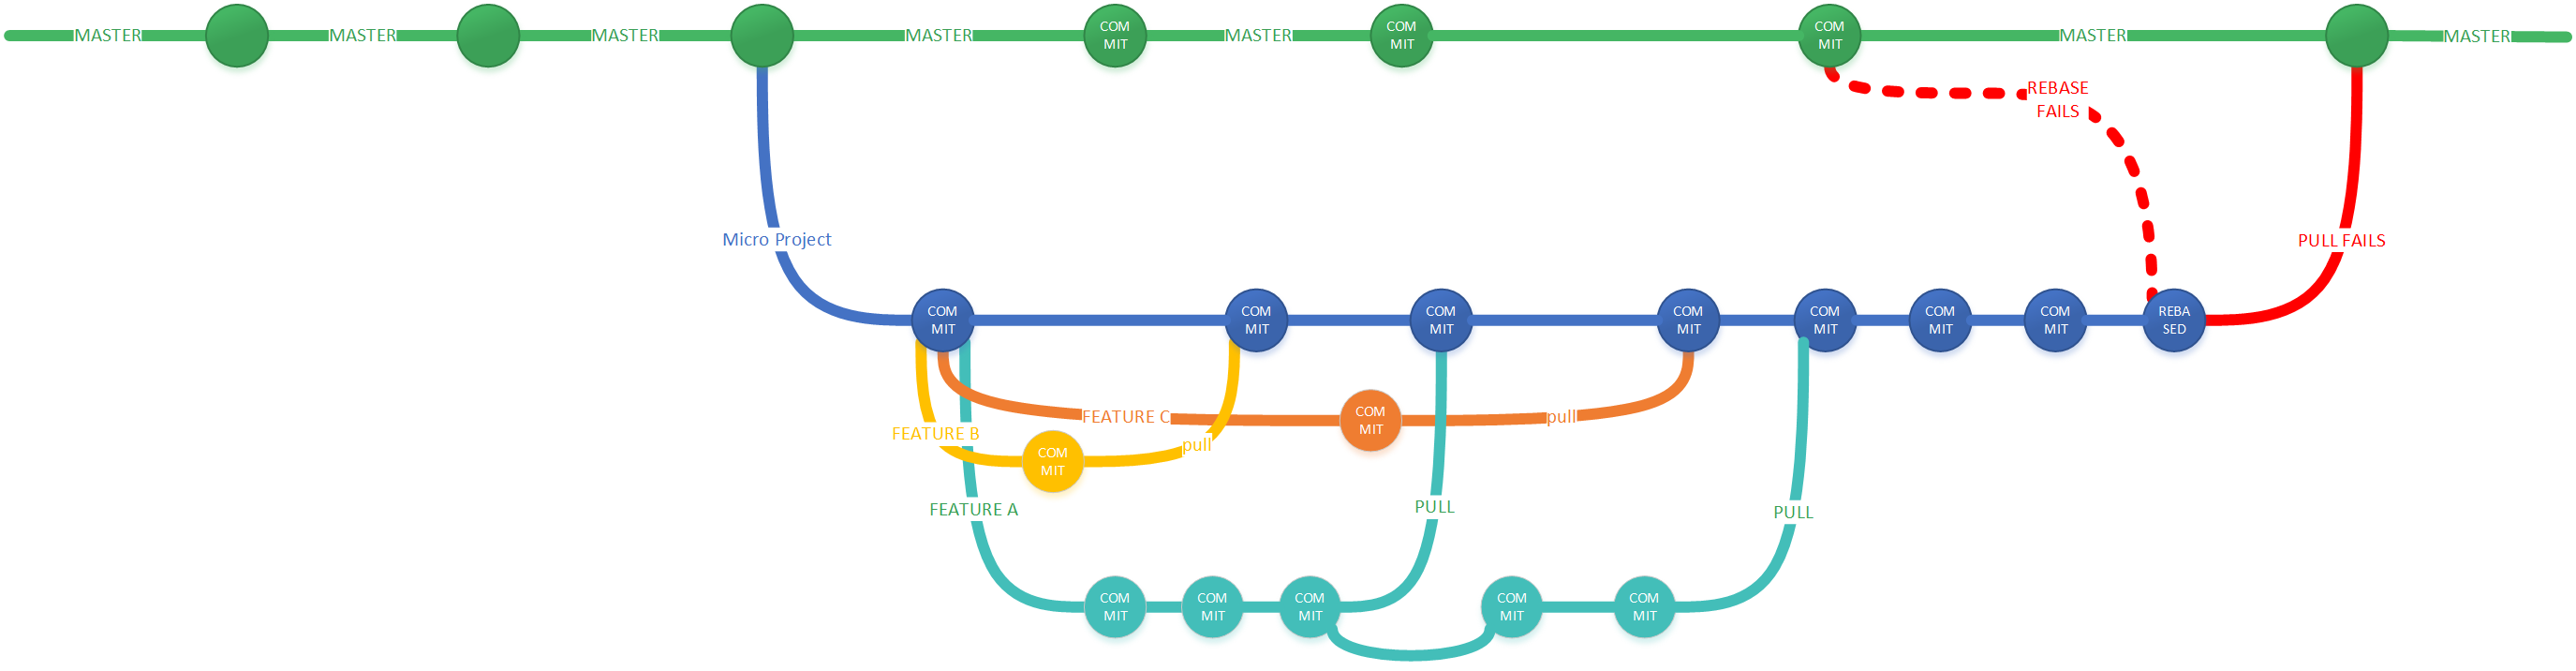
\includegraphics[width=\textwidth]{img/branch.png}
\caption{Git branches}
\label{fig:branches}
\end{figure}

\paragraph{}
Once the task is finished passing all integration and acceptance tests, moved into the DONE state. Before a task can be put into the Done state the developer assigned to the task, must create a Pull Request for the task, which in turn will be reviewed by their colleagues / management to confirm that the task meets the specification of the task, conforms to the quality requirements expected, and works as expected\cite{driessen}.

\chapter{Technology Review}
About seven to ten pages.
\begin{itemize}
\item Describe each of the technologies you used at a conceptual level. Standards, Database Model (e.g. MongoDB, CouchDB), XMl, WSDL, JSON, JAXP.
\item Use references (IEEE format, e.g. [1]), Books, Papers, URLs (timestamp) – sources should be authoritative. 
\end{itemize}

\section{Docker}

\subsection{What is Docker?}
Docker is a platform that enables containerization of applications. Containerization provides standardized units for development, shipment and deployment. Container images are lightweight, isolated, executable packages of software that contain all the components to run the specified; the code, tools, dependencies, and settings. With availability on Linux and Windows based containers, both will run seamlessly regardless of the environment. Containers running in isolation means that regardless of how the environment or infrastructure which the container will run on, the application within the container will be unaffected by discrepancies across the environments, and other applications. Docker provides containers that run on a single machine share the operating system-kernel, resulting in rapid starting and less consumption of the central processing unit (CPU) and random access memory (RAM). Based on open standards, Docker containers can run on all major Linux distributions, Microsoft Windows, Apple MAC OS, and any infrastructure like: virtual machines, bare-metal, and via cloud services. 

\subsection{Docker Containers v Virtual Machines}
What are the benefits or differences of using Docker containers over Virtual Machines? 
While Docker containers and virtual machines have relatively similar resource isolation and allocation benefits, they function differently. Where a virtual machine will mimic the behavior of an operating system running on a physical computer, Docker containers visualizer just the operating system, rather than the operating system running on the hardware itself, resulting in higher efficiency and portability. Consider figure \ref{fig:containervsvm}

\begin{figure}
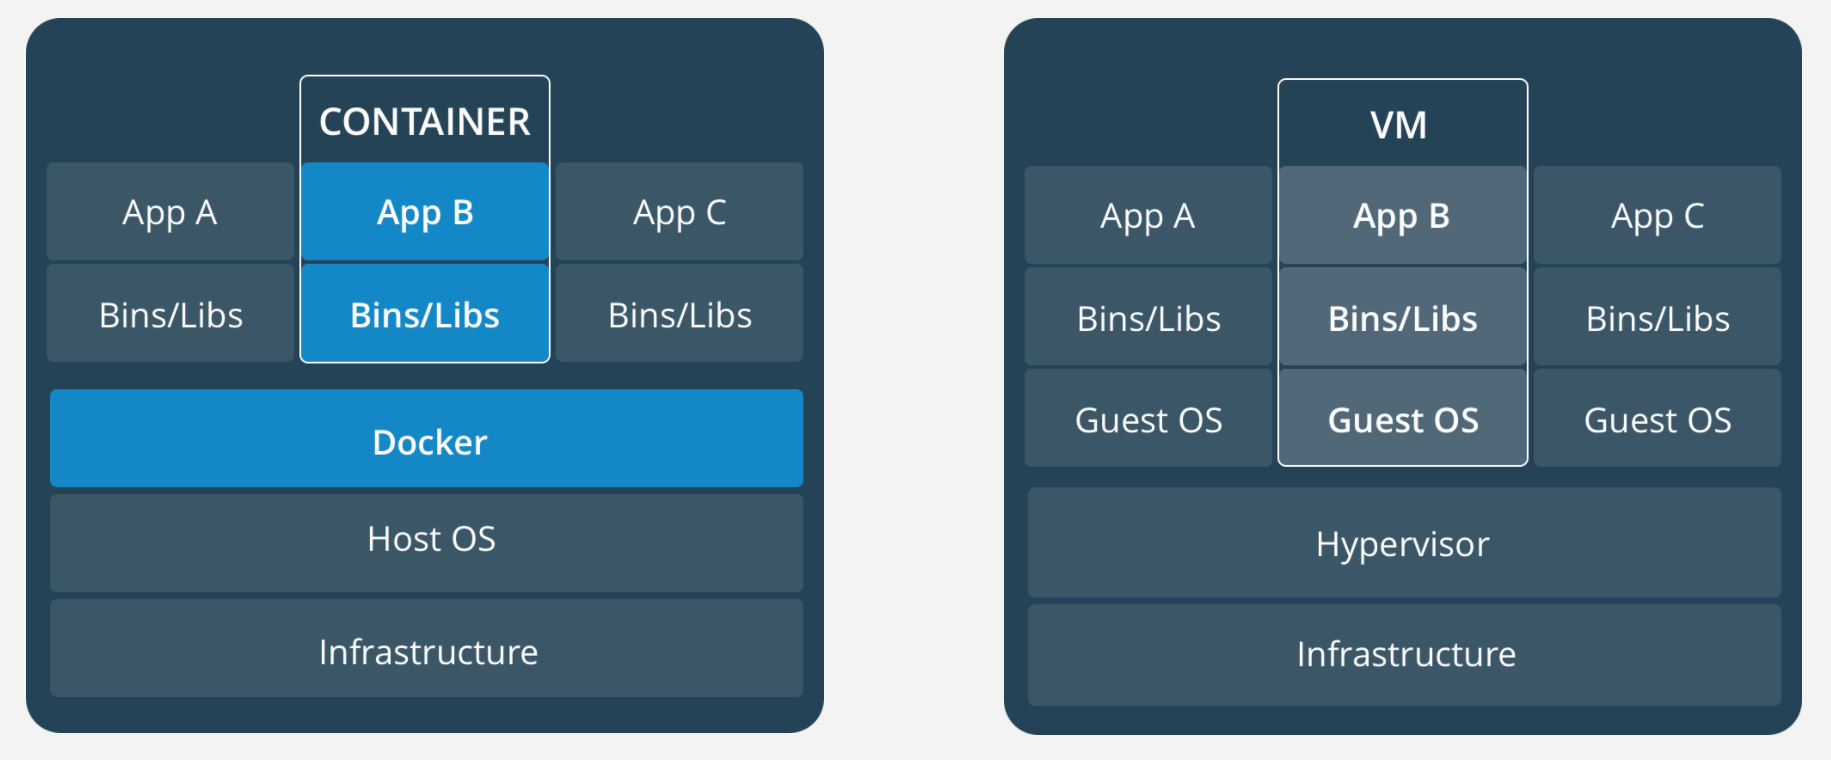
\includegraphics[width=\textwidth]{img/containervvm.PNG}
\caption{Docker Containers vs Virtual Machines}
\label{fig:containervsvm}
\end{figure}

Containers are an abstraction at the application layer which packages the code and dependencies  together. Numerous Docker containers can be running on the same machine and share resources such as the operating system kernel with other Docker containers running on the same machine, even though each of these Docker containers are running in isolation in the user space. Docker containers also require less space than virtual machines, with a container image typically using less than one hundred megabytes of storage space in size, alongside their near immediate start time.
On the other hand Virtual machines, are an abstraction of physical hardware allowing one server to appear or act as if it were many servers. The hyper-visor, also known as virtual machine monitor, produces any guest operating systems with a virtual operating platform and in turn manages the execution of all guest operating systems on the host machine. Each virtual machine will have a full copy of an operating system, one or many applications, any required dependencies, libraries and binaries, all of which would consume up to or more than one hundred gigabytes. Virtual machines can also be slow to launch. 

Docker is a container platform to construct, secure and administer a large array of applications from the early stages of development to deployment and production whether they are local or “in the cloud”. Docker Community Edition provides tools to build applications to developers for free, whereas Docker Enterprise Edition provides a Containers-as-a-Service platform for IT companies with multi-architecture operations at scale. 

\subsection{Dockerizing Existing Applications}
An application does not have to be built from the ground up with Docker, as existing applications  can be containerized. With potential of reducing cost, start up time, and provide a layer of security, Docker can aid in time and resource management when building new applications or even modernizing legacy applications. Using the Modernize Traditional Applications [MTA] kit via Docker Enterprise Edition, developers can package existing applications into containers, which will enable the application to be portable. This alteration implements modern properties to legacy applications, without the need to change any of the source code. It will also reduce the overhead required to run the legacy application, increase operational efficiency, and consolidate infrastructure.

Because Docker packages applications and their dependencies together into an isolated container, this makes them portable to any infrastructure, making them suitable for Cloud migration, multi-cloud or hybrid cloud infrastructures. Thus eliminating the age-old “works on my machine” problem. The Docker Certified Infrastructure guarantees that the containerized applications work consistently. It provides an integrated environment for multiple distributions of enterprise Linux, as well as on Cloud providers such as Amazon Web Services, Azure and IBM. Docker Certified containers provide trusted independent software vendor products packaged and distributed via Docker containers. Docker Certified plug ins provide easy to download and install containers for an environment, as well as networking and volume plug ins.

\subsection{Continuous Integration and Services}
Docker also provides tools and strategies to Developer Operations (Dev Ops) teams. John Willis’ White paper on “Docker and the Three Ways of DevOps“, outline three principles known as “The Three Ways of DevOps”, and describes the purpose of these principles, how to apply these principles using Docker within organizations, and the results and benefits from doing so. 

\textbf{\emph{“The First Way: System Thinking”}}

This is referred to as the pipeline; the flow and direction from left to right, outlining the importance of understanding the system as a complete value stream. Managing this concept is often referred to as bottleneck reduction or global optimization, or “Lead Time” in the Lean project management methodology\cite{willis}. This is the equivalent of the time taken to get from rough diagrams to the delivery of a product to paying consumers, or in simpler terms, the time from starting a project, and the project becoming a product of value\cite{willis}.  To ensure System Thinking is effective, Dev Ops teams need to able to apply the following:

\begin{itemize}
\item Escalate “velocity” by hastening each process component within the pipeline.
\item Diminish “variation” by removing wasteful or time intensive sub processes within the pipeline.
\item Ascension of processes by isolating functionality, therefore improving visualization and understanding of the overall flow.
\end{itemize}

Docker can aid the above in the following ways:
\begin{itemize}
\item \textbf{Velocity:}
	\begin{itemize}
	\item In regards to \emph{Development flow}, developers using Docker can create Docker environments locally on their machine to develop and test containerized applications. In contrast, the alternative of using virtual instances running as numerous hosts could consume a lot of time during start up time and convergence, depending on the overall complexity\cite{willis}. To summarize, Docker delivers less context switching time for testing and retesting, resulting in significantly higher velocity.
    \item In regards to \emph{Integration flow}, Docker can simplify continuous integration with use of Dockerized build slaves.  A continuous integration system can be designed in such a way that it would allow multiple virtual instances to run in isolation, each as individual hosts. Environments can run Docker hosts within a Docker host, termed “Docker-in-Docker” for build environments. This provides elegant isolation of the build and breaks down the environments for the services in test, meaning that the original instances are never debased due to the embedded host having the ability to be recreated for each slave instance\cite{willis}. 
    \item Finally with regards to \emph{Deployment flow}, to achieve higher velocity in  Continuous Delivery of software, there are numerous approaches that may be hit by using Docker. One challenge of production deployments is ensuring the seamless and quick changeover time from version to version. "A Blue Green deploy is a technique where one node of a cluster is updated at a time (i.e., the green node) while the other nodes are still untouched (the blue nodes)."\cite{willis} This approach requires a continuous process where each node is updated and tested, one at a time. The fundamental outcomes  of this are:
	\begin{enumerate}
		\item The time required to update all nodes needs to be fast.
    	\item If a cluster requires roll back, this must also be done fast.  
	\end{enumerate}
    To summarize, Docker containers execute the roll back and roll forward processes more efficiently, and also are a lot cleaner due to container isolation during changeover.
	\end{itemize}
\item \textbf{Variation:}
	A fundamental pro of using Docker images throughout the software delivery pipeline is that the environment and application can both be packaged within the container image. With Docker, a developer can package the actual environment (e.g OS, dependencies, other requirements) within the same image. This convergence reduces the possible variation at all stages of the delivery pipeline; i.e. development, integration, and  deployment\cite{willis}. If a developer were to test a collection of Docker images as a service on any machine, the services in question can be the exact same during integration testing and right up to deployment. "A Dockerized pipeline approach delivers converged artifacts as binaries and therefore are immutable starting from the commit"\cite{willis}.
\item \textbf{Visualization}
	Containerized Microservices is a model which has been generating a buzz within the software development world lately. In an architecture of micro services, “services” are defined as bounded context. When these services are connected as Docker containers and used within the delivery pipeline, they become visible without delay on a domain. Services become more visible in the pipeline when bounded by their business context and then isolated as Docker containers. With more visibility an organization can isolate, and determine control rapidly; thus reducing overall Mean time to repair\cite{willis}.
    "The “First Way”” and Docker can provide global optimization around software Velocity, Variation and Visualization. Dockerizing the development pipeline, organizations can reduce the cost and risk of software delivery while increasing the rate of change."\cite{willis} 
\end{itemize}

\textbf{\emph{"The Second Way: Amplify Feedback Loops"}}

"The "Second Way" is defined as amplifying and shortening feedback loops such that connections can be made fast and continuously."\cite{willis} also known as the right to left flow.

\begin{itemize}
\item \textbf{Velocity}
	In the second way velocity means the same as Velocity from the first way. The flow in this case may not always be going in the same direction. Defect cause interruptions in the flow and changeover time. Dev Ops need to manage, feedback, changeover speed, the adaptiveness of the system in relation to defect detection, and reimplementation. Dockers streamlining of packaging allows organizations to utilize shorter changeover times because of defects, making it easier to halt processes if any defects are indeed identified.\cite{willis}
    \item \textbf{Visualization}
    An advantage of the immutable delivery process is most artifacts are conveyed throughout the pipeline as binaries\cite{willis}. This means that service delivery teams are able to generate meta-data from the source that is maintained, enabling visualization at any stage within the pipeline. With that meta-data the time required to resolve defects is reduced, therefore the overall Lead Time of the service being delivered is also reduced. 
\end{itemize}

\textbf{\emph{"The Third Way: Continuous Learning"}}

"In this “Third Way”, the symbol of a complete loop is used because it ties the first two ways together through a rigorous implementation of a learning process."\cite{willis} The word Kaizen is often seen as an approach of continuous improvement within an organization. This approach being fulfilled through a culture of continuous experimentation and learning in all parts of the organization\cite{willis}. The speed to market is essential in the deliverance of software and services. It is also the speed at which reaction, and reproduction to customers validation of the delivered service. The major principles of the Dev Ops mindset all point to outcomes like rapid innovation, increased quality and a feedback loop of continuous learning. "The Docker platform uniquely allows organizations to apply tools into their application environment to accelerate the rate of change, reduce friction and improve efficiencies."\cite{willis}.

\subsection{Conclusion}
	To summarize, Docker as a development tool is relatively easy to pick up and implement, due to the fact that it is well supported and documented by its community. However, it comes with a steep learning curve as you traverse deeper into its more advanced features and functionality. The isolated environments that Docker containers provide, enables work across different machines regardless of the underlying infrastructure, which in the case of this project, provided an easy work flow during cross examination, merging, and service integration. Going forward Docker will continue to make this project more and more versatile, secure, quick, and easy to maintain because of the Docker ethos. Long after the project has been deployed and it is in use by the product owner, integration engineers and developer operations teams should find processes like: onboarding new services, or analyzing and repairing problematic services easy to identify, then address, seamlessly and fast. Finally with the exponential growth in adoption rate of Docker over the last couple of years, virtual machines may very well be a thing of the past in years to come.

\section{NodeJS}
\subsection{About Node}
	Node is designed as an asynchronous event driven JavaScript runtime for scalable network applications built off Google Chrome V8 Engine. Google Chrome V8 Engine will translate the JavaScript, which Node API's are written in, into machine readable code. Node provides the ability to handle many connections concurrently using callbacks, but if there is no work pending, it will sleep\cite{nodejs}. This is in opposition to the current common concurrency model that employs operating system threads, as thread-based networking can be relatively difficult to use and inefficient. Node users need not worry of processes dead-locking, since no locks exist. I/O processes never block, because very few functions in Node directly perform I/O, as a result of this scalable systems are feasible to build using Node. Node presents an event loop as a runtime construct rather than as a library. Node will enter this event loop after execution of an input script, and exit the event loop once all callbacks have been performed\cite{nodejs}.
    
\subsection{JavaScript to Machine Code via the Google Chrome V8 Engine}
	\subsubsection{What is it?}
    	The V8 Engine is an open source high-performance JavaScript engine from Google, written in C++ that is used in Google Chrome, NodeJS, and more. The V8 Engine can be embedded into any C++ application or run standalone\cite{googleV8}. \emph{"V8 implements ECMAScript as specified in ECMA-262, 5th edition, and runs on Windows (XP or newer), Mac OS X (10.5 or newer), and Linux systems that use IA-32, x64, or ARM processors."}\cite{googleV8} 
	\subsubsection{How does it work?}
    The V8 Engine is capable of compiling and executing JavaScript source code, handling allocation of memory for objects, as well as garbage collection for redundant objects that are no longer needed. This garbage collector is key to the V8 Engines performance. Designed specifically for quick execution of large JavaScript applications, there are three primary areas tied to the V8 Engines performance: 
    \begin{enumerate}
    \item Fast Property Access
    	\begin{itemize}
    	\item With JavaScript's dynamic nature, the properties of objects can be added or removed while in progress, which means that they are likely to change. To reduce the time complexity of accessing JavaScript properties, the V8 Engine dynamically creates hidden classes in the background. When a property is added or removed this hidden class will be updated, rather than using a dynamic lookup to resolve the property's location in memory\cite{googleV8}. \emph{"There are two advantages to using hidden classes: property access does not require a dictionary lookup, and they enable V8 to use the classic class-based optimization, inline caching."}\cite{googleV8} 
    	\end{itemize}
    \item Dynamic Machine Code Generation
    	\begin{itemize}
    	\item The V8 Engine will determine the state of an object's current hidden class at initial code execution for property access of any given object. Property access is optimized by prediction of future use of a class for any future objects accessed in the same code section and usage of information from the class to patch inline cached code used to the hidden class\cite{googleV8}. \emph{"The combination of using hidden classes to access properties with inline caching and machine code generation optimises for cases where the same type of object is frequently created and accessed in a similar way. This greatly improves the speed at which most JavaScript code can be executed."}\cite{googleV8}
    	\end{itemize}
    \item Efficient Garbage Collection
    	\begin{itemize}
    	\item The V8 Engine will garbage collect objects that are no longer needed, reclaiming the memory used by said objects. The V8 Engine uses a \emph{"stop-the-world, generational, accurate, garbage collector"}\cite{googleV8} to make sure that object allocation is fast, garbage collection is short, and no memory fragmenting occurs.
    	\end{itemize}
    \end{enumerate}
    
    
    	

\subsection{The Event Loop}

\subsection{Typescript integration with NodeJS}

\subsection{Conclusion}





	




\section{XML}
Here's some nicely formatted XML:
\begin{minted}{xml}
<this>
  <looks lookswhat="good">
    Good
  </looks>
</this>
\end{minted}

\chapter{System Design}
As many pages as needed.
\begin{itemize}
\item Architecture, UML etc. An overview of the different components of the system. Diagrams etc… Screen shots etc.
\end{itemize}

\begin{table}[h]
  \centering
  \begin{tabular}{x{2cm}p{3cm}}
    \toprule \\
    Column 1 & Column 2 \\
    \midrule \\
    Rows 2.1 & Row 2.2 \\
    \bottomrule
  \end{tabular}
  \caption{A table.}
  \label{table:mytable}
\end{table}

\chapter{System Evaluation}
As many pages as needed.
\begin{itemize}
\item Prove that your software is robust. How? Testing etc. 
\item Use performance benchmarks (space and time) if algorithmic.
\item Measure the outcomes / outputs of your system / software against the objectives from the Introduction.
\item Highlight any limitations or opportuni-ties in your approach or technologies used.
\end{itemize}

\chapter{Conclusion}
About three pages.

\begin{itemize}
\item Briefly summarise your context and ob-jectives (a few lines).
\item Highlight your findings from the evaluation section / chapter and any opportuni-ties identified.
\end{itemize}

\chapter{Appendix}
\begin{itemize}
\item \textbf{Source code Git Repository:} \url{https://bitbucket.org/deltaready-mcs/mcs-microservices-mono-repo}
\item \textbf{Dissertation Git Repository:} \url{https://github.com/Verdagio/Final-Year-Minor-Dissertation}
\end{itemize}







